\documentclass{beamer}

\usepackage{graphicx}
\usetheme{Szeged}
\usecolortheme{beaver}

\author{Anne Wanningen \and Xeryus Stokkel}
\title[Week 6]{Introduction to Computer Graphics Raytracer week 6}

\begin{document}

\maketitle

\section{Gooch Shading}

\begin{frame}
	\begin{columns}[T]
		\begin{column}{.3\textwidth}
			\begin{figure}
				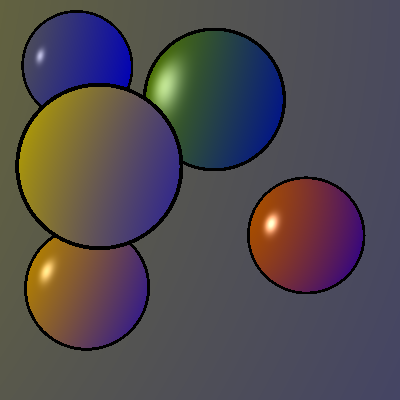
\includegraphics[width=\textwidth]{ref.png}
			\end{figure}
		\end{column}
		\begin{column}{.3\textwidth}
			\begin{figure}
				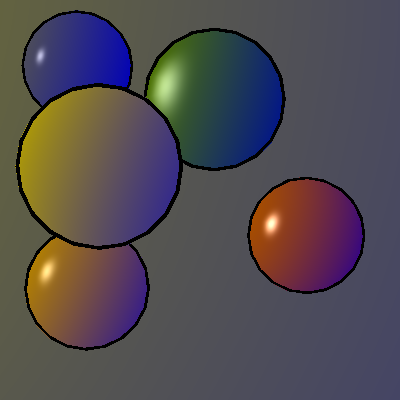
\includegraphics[width=\textwidth]{res.png}
			\end{figure}
		\end{column}
		\begin{column}{.3\textwidth}
			\begin{figure}
				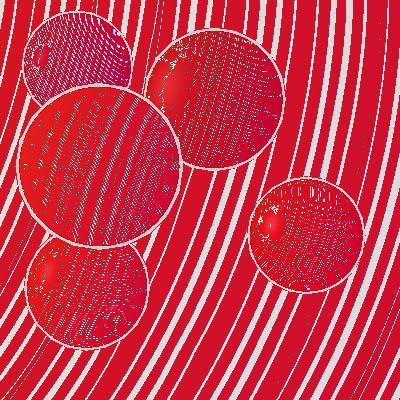
\includegraphics[width=\textwidth]{diff.png}
			\end{figure}
		\end{column}
\end{columns}
\end{frame}
\end{document}
